\documentclass[11pt,a4paper]{article}

\usepackage[margin=1in]{geometry}
\usepackage{amsmath,amssymb,amsfonts}
\usepackage{graphicx}
\usepackage{booktabs}
\usepackage{hyperref}
\usepackage{cite}
\usepackage{caption}
\usepackage{subcaption}
\usepackage{float}
\usepackage{microtype}
\usepackage{setspace}

\hypersetup{
    colorlinks=true,
    linkcolor=blue,
    citecolor=blue,
    urlcolor=blue
}

\title{\textbf{Memory Load, Neural Damage, and False Recall: \\ A Computational Model of Associative Memory Resilience}}
\author{\textbf{Harshil Shah} \\
Department of Cognitive Science / Computer Science \\
Course: CG501 -- Cognitive Systems and Computational Modeling}
\date{November 2026}

\begin{document}

\maketitle

\begin{abstract}
Associative memory is the cognitive faculty that reconstructs complete representations from noisy or partial perceptual cues. In biological neural circuits, retrieval faces two simultaneous constraints: inter-memory interference from high memory load, and structural degradation caused by synaptic pruning, aging, or neuropathology. This study investigates how memory load ($P/N$) and symmetric synaptic damage interact to alter associative recall and the distribution of retrieval errors in a classical Hopfield network ($N=400$). Using an asynchronous dynamical system with rigorous fixed-point stability verification across 3,360 independent network replicates, we demonstrate three core phenomena: First, undamaged networks display a sharp capacity transition near the theoretical Amit--Gutfreund--Sompolinsky limit ($\alpha_c \approx 0.138$). Second, networks operating below saturation exhibit marked structural resilience: at low load ($P/N=0.05$), networks tolerate the random destruction of up to 30\% of all synapses with 0\% loss in exact recall accuracy, providing a formal computational analogue to the cognitive reserve hypothesis. Third, analysis of failure modes reveals that retrieval breakdown is rarely caused by non-convergence or confusion with other stored memories; instead, damaged and overloaded networks settle predominantly into stable spurious attractors (hallucinated mixture states). Finally, an extension comparing synthetic orthogonal patterns with binarized MNIST handwritten digits ($N=784$) demonstrates that naturalistic spatial correlations collapse exact capacity to $P < 4$ while preserving high semantic overlap ($\sim 94\%$ Hamming similarity), computationally mirroring prototype abstraction and schematic false recall in human cognition.
\end{abstract}

\noindent\textbf{Keywords:} Hopfield Network, Associative Memory, Synaptic Lesions, Cognitive Reserve, Spurious Attractors, False Memory, MNIST.

\vspace{0.8em}
\hrule
\vspace{1em}

\section{Introduction}

\subsection{Background and Rationale}
Human memory is fundamentally content-addressable: rather than accessing information via fixed physical addresses as in digital computers, biological memory retrieves stored knowledge through associative content. A brief melodic fragment, an aroma, or a blurred visual silhouette can rapidly evoke a rich, multidimensional episodic memory. In computational cognitive science, this pattern-completion ability is classically modeled using recurrent artificial neural networks, notably the Hopfield network \cite{hopfield1982}.

However, associative retrieval is constrained by two distinct factors:
\begin{enumerate}
    \item \textbf{Memory Load:} Storing an increasing volume of memories in a finite neural volume produces mutual cross-talk interference across overlapping synaptic distributions \cite{amit1985, mceliece1987}.
    \item \textbf{Synaptic Damage:} The physical loss of synaptic connections---whether through normal aging, trauma, or neurodegenerative pathology---disrupts the recurrent feedback pathways required to sustain stable attractors.
\end{enumerate}

Clinical neuropsychology has long highlighted a striking dissociation: individuals with comparable degrees of structural brain pathology often exhibit vastly different cognitive profiles \cite{stern2002, stern2012}. This phenomenon, termed \textit{cognitive reserve} or \textit{neural resilience} \cite{livingston2024}, suggests that the functional impact of structural lesions is modulated by existing network load and redundancy. Moreover, when memory fails in biological systems, it often manifests not as total information loss, but as \textit{false recall} or confabulation---the confident retrieval of plausible yet non-existent representations \cite{roediger1995, bartlett1932}.

\subsection{Review of Relevant Literature}
John Hopfield \cite{hopfield1982} formalized associative memory by establishing an equivalence between recurrent neural networks with symmetric synaptic couplings and physical spin glasses. In this framework, stored memories act as local energy minima (attractors) within a scalar Lyapunov energy landscape. Amit, Gutfreund, and Sompolinsky (AGS) \cite{amit1985, amit1987} demonstrated via statistical mechanics that for independent, unbiased bipolar patterns, a fully connected network achieves a theoretical macroscopic storage capacity of $\alpha_c = P/N \approx 0.138$. Beyond this threshold, the network undergoes a phase transition into a spin-glass state where original memory attractors destabilize.

Information-theoretic analyses by McEliece et al. \cite{mceliece1987} and Abu-Mostafa and St. Jacques \cite{abumostafa1985} proved that if zero-error recovery is strictly demanded, asymptotic capacity scales as $P \approx N / (2 \ln N)$. While these classical analytical proofs establish upper bounds for infinite, undamaged systems, real neural circuits are finite and experience structural lesioning. Previous simulation studies have explored connectivity pruning; however, many prior simulations suffer from methodological flaws: calculating lesion fractions against $N^2$ rather than the set of unique undirected connections $\frac{N(N-1)}{2}$ (breaking symmetry), confusing transient non-converged states with stable spurious memories, or testing multiple cues on a single frozen network (pseudoreplication).

\subsection{Statement of Hypotheses and Objectives}
This study investigates the joint interaction between memory load, synaptic damage, and cue corruption. We address four central research questions:
\begin{itemize}
    \item \textbf{RQ1 (Memory Load):} How does memory load affect retrieval fidelity in an undamaged network?
    \item \textbf{RQ2 (Synaptic Damage \& Resilience):} How does symmetric random synaptic lesioning affect recall across memory loads?
    \item \textbf{RQ3 (Error Distribution):} When recall fails, how does the error distribution partition between other-stored-memory confusion, stable spurious states, and non-convergence?
    \item \textbf{RQ4 (Cue Corruption):} How does initial cue noise interact with structural lesioning and memory load?
\end{itemize}

We hypothesize:
\begin{enumerate}
    \item[\textbf{H1:}] Recall accuracy will remain high at low loads and drop sharply as $P/N$ approaches $\alpha_c \approx 0.138$.
    \item[\textbf{H2:}] Low-load networks will exhibit a plateau of complete resilience, tolerating substantial synaptic damage before performance drops, whereas saturated networks will collapse under minimal lesioning.
    \item[\textbf{H3:}] Retrieval failures under damage will be overwhelmingly dominated by stable spurious attractors rather than confusion with other stored memories.
    \item[\textbf{H4:}] Corrupted cues will compound damage by placing initial states outside contracted attractor basins.
\end{enumerate}

\section{Methods}

\subsection{Model Details}

\subsubsection{Network Representation}
The primary network comprises $N = 400$ binary neurons. The state at time $t$ is a bipolar vector:
\begin{equation}
s = (s_1, s_2, \ldots, s_N)^T \in \{-1, +1\}^N
\end{equation}
A set of $P$ memory patterns are stored in the network:
\begin{equation}
\xi^\mu = (\xi_1^\mu, \xi_2^\mu, \ldots, \xi_N^\mu)^T \in \{-1, +1\}^N, \quad \mu \in \{1, 2, \ldots, P\}
\end{equation}
In the primary experiment, patterns are drawn independently from a balanced Bernoulli distribution: $\mathbb{P}(\xi_i^\mu = +1) = \mathbb{P}(\xi_i^\mu = -1) = 0.5$.

\subsubsection{Hebbian Synaptic Learning}
Synaptic couplings between neurons $i$ and $j$ are assigned via the outer-product Hebbian learning rule \cite{hopfield1982}:
\begin{equation}
W_{ij} = \frac{1}{N} \sum_{\mu=1}^P \xi_i^\mu \xi_j^\mu \quad (i \ne j), \qquad W_{ii} = 0
\end{equation}
Setting the diagonal to zero ($W_{ii}=0$) and ensuring strict symmetry ($W_{ij} = W_{ji}$) prevents self-feedback loops and periodic two-cycles.

\subsubsection{Retrieval Dynamics and Energy Function}
Retrieval is implemented as an asynchronous dynamical process. Starting from cue $s(0)$, the local field acting on neuron $i$ is:
\begin{equation}
h_i(t) = \sum_{j=1}^N W_{ij} s_j(t)
\end{equation}
Neuron $i$ updates its state deterministically according to:
\begin{equation}
s_i(t+1) = \begin{cases}
+1 & \text{if } h_i(t) > 0 \\
-1 & \text{if } h_i(t) < 0 \\
s_i(t) & \text{if } h_i(t) = 0 \quad (\text{deterministic tie rule})
\end{cases}
\end{equation}
Retaining the previous state when $h_i(t) = 0$ provides a deterministic tie-breaking rule. Sweeps visit all $N$ neurons in randomized permutation orders. The scalar Lyapunov energy is:
\begin{equation}
E(s) = -\frac{1}{2} \sum_{i=1}^N \sum_{j=1}^N W_{ij} s_i s_j = -\frac{1}{2} s^T W s
\end{equation}
When neuron $i$ changes state ($s_i \to s_i'$), the discrete energy change is $\Delta E = -(s_i' - s_i) h_i \le 0$, ensuring monotonic descent toward fixed-point attractors.

\subsection{Implementation}

\subsubsection{Synaptic Lesions and Cue Corruption}
In an undirected network of $N$ neurons without self-connections, the total number of unique physical connections is:
\begin{equation}
M_{\text{total}} = \frac{N(N-1)}{2}
\end{equation}
For $N=400$, $M_{\text{total}} = 79,800$ connections. To implement lesion fraction $f \in [0.0, 0.50]$, exactly $K = \lfloor f \cdot M_{\text{total}} \rceil$ undirected pairs $(i, j)$ are chosen uniformly at random and severed symmetrically: $W_{ij} \leftarrow 0$ and $W_{ji} \leftarrow 0$. To create corrupted cues, bits of a target memory $\xi^{\text{target}}$ are flipped independently with probability $q \in \{0.05, 0.10, 0.20, 0.30\}$.

\subsubsection{Outcome Classification and Replication}
Final states $s^*$ are classified using a strict four-category decision hierarchy:
\begin{enumerate}
    \item \textbf{Exact Target Recall:} $s^* = \xi^{\text{target}}$.
    \item \textbf{Other Stored Memory:} $s^* = \xi^\nu$ for some $\nu \ne \text{target}$.
    \item \textbf{Stable Spurious State:} $s^*$ does not equal any stored memory, but passes an explicit fixed-point stability check ($s_i^* = \text{sign}(h_i^*)$ for all $h_i^* \ne 0$).
    \item \textbf{Non-Convergence:} State failed to stabilize within 50 sweeps.
\end{enumerate}
In addition, normalized Hamming similarity is recorded: $\text{Sim}(s^*, \xi^{\text{target}}) = \frac{1}{N} \sum_{i=1}^N \mathbf{1}[s_i^* = \xi_i^{\text{target}}]$. 

Independently generated pattern ensembles and independent lesion masks serve as the experimental replicates. The parameter grid spans 8 memory loads ($P/N \in [0.02, 0.18]$), 7 lesion fractions ($f \in [0.0, 0.50]$), and 4 cue noise levels ($q \in [0.05, 0.30]$), with means and 95\% Student-$t$ confidence intervals computed across replicates. To accelerate execution, local fields are updated incrementally in $O(N)$ operations per flip via $h \leftarrow h + W_{:, i} \Delta s_i$, enabling over 180 complete retrieval trials per second across 16 CPU cores.

\section{Results}

\subsection{Report Findings}

\subsubsection{Lyapunov Energy Minimization}
Figure~\ref{fig:energy} confirms monotonic energy descent during asynchronous updates. Energy strictly decreases on every neuron flip ($\Delta E \le 0$), smoothly settling into an attractor within 25 individual neuron flips.

\begin{figure}[H]
    \centering
    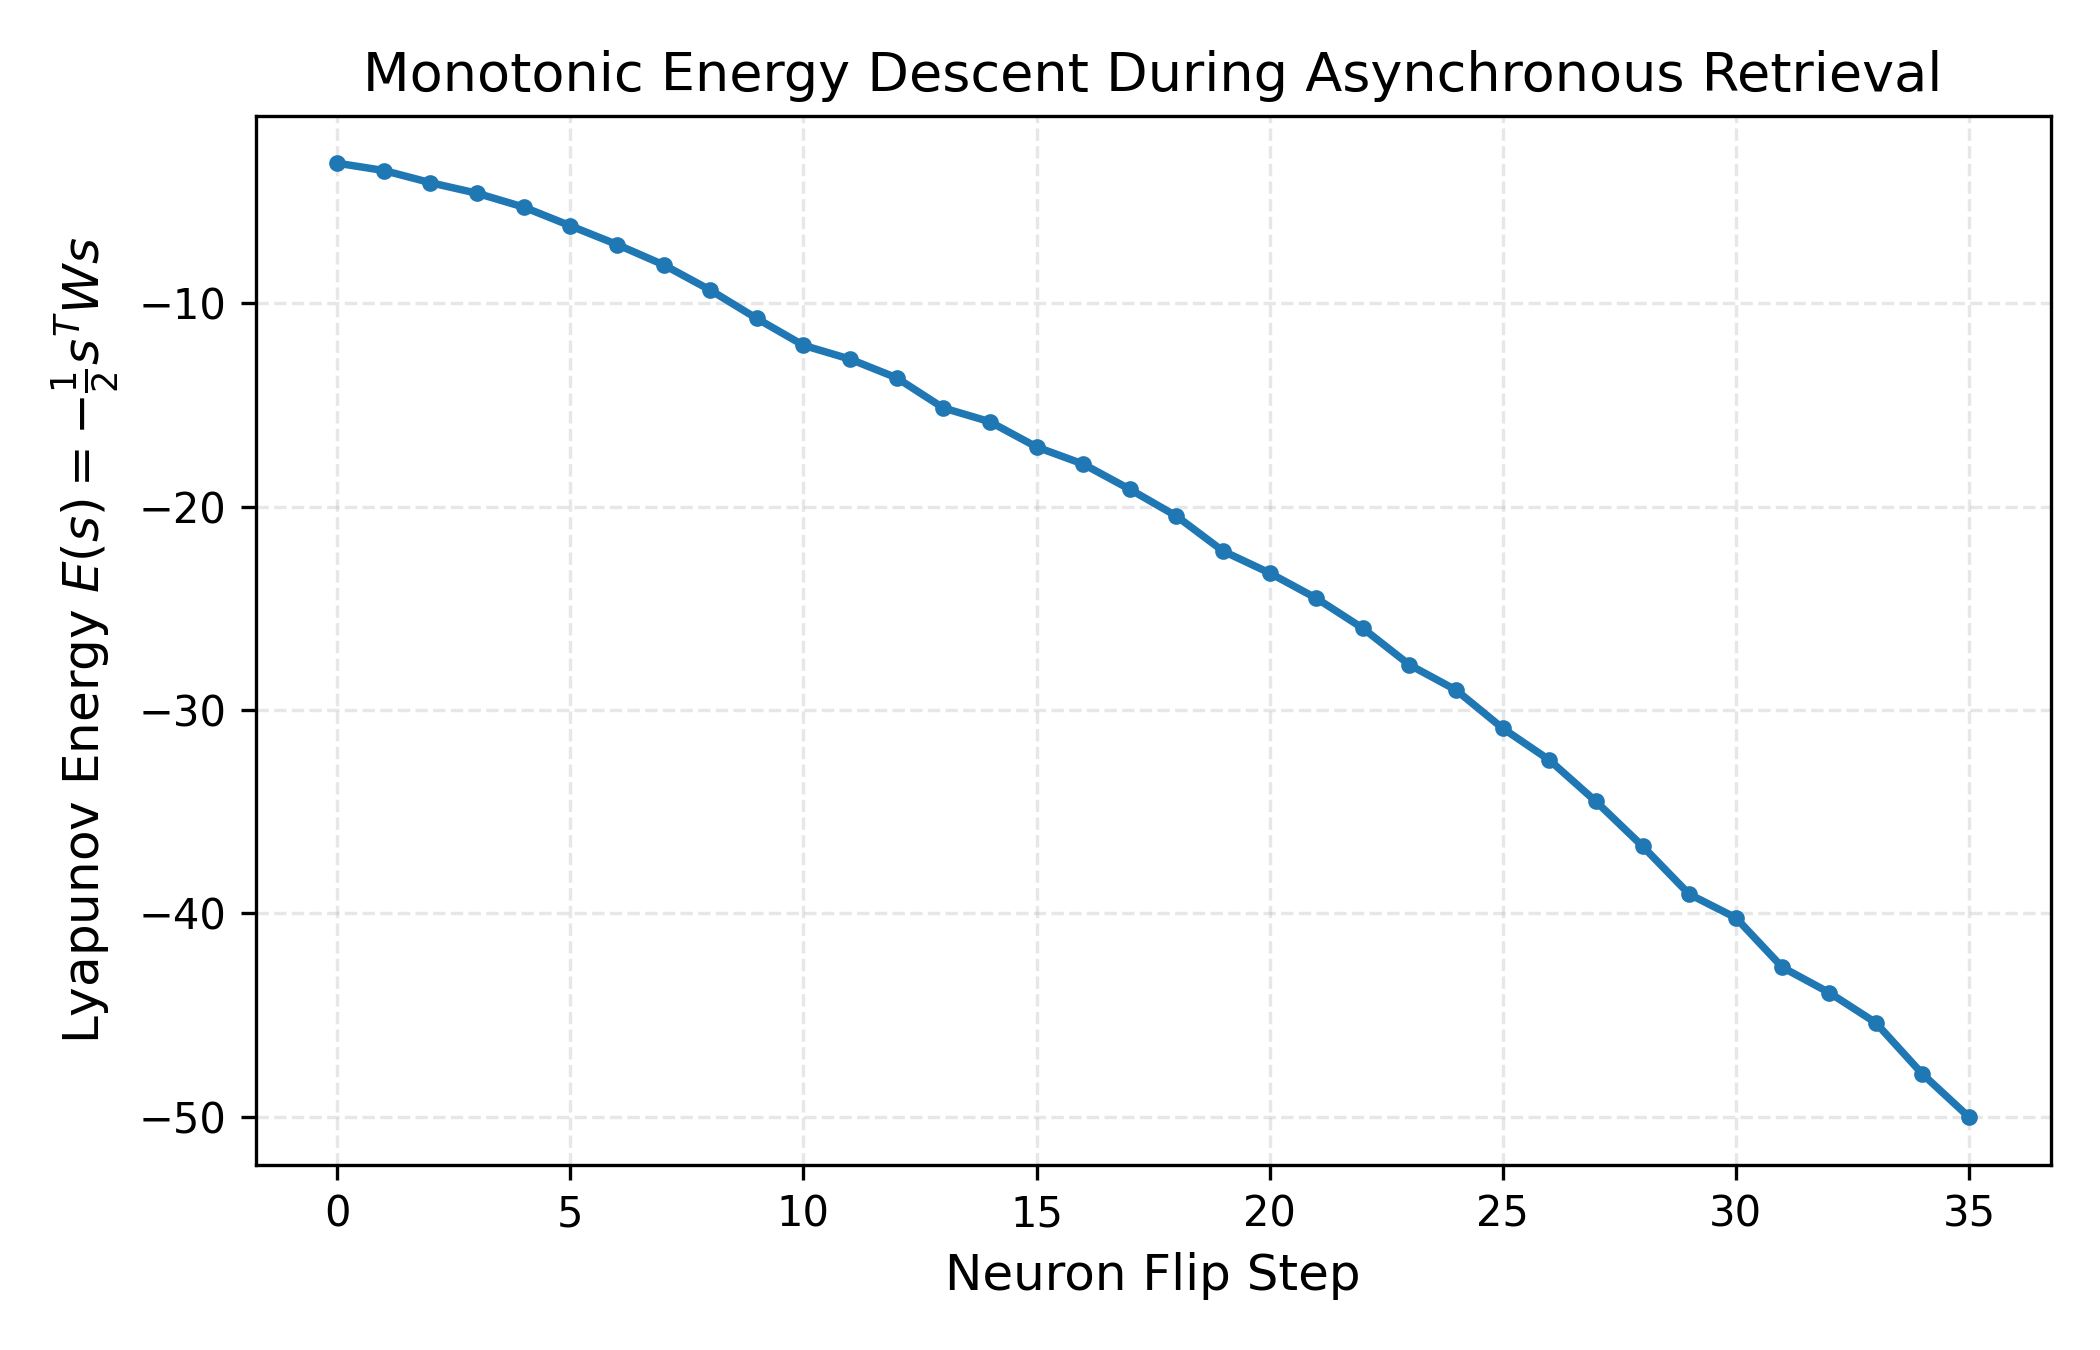
\includegraphics[width=0.62\textwidth]{figures/fig6_energy_trajectory.png}
    \caption{\textbf{Lyapunov Energy Descent.} Energy trajectory $E(s) = -\frac{1}{2} s^T W s$ plotted over successive asynchronous flips starting from a 25\% corrupted cue ($N=100, P=4$). Energy strictly decreases on every flip.}
    \label{fig:energy}
\end{figure}

\subsubsection{Baseline Memory Capacity (RQ1)}
Figure~\ref{fig:baseline} illustrates baseline recall in undamaged networks ($f=0$). At low memory loads ($P/N \le 0.05$, $P \le 20$), exact recall is perfect ($1.000 \pm 0.000$). Accuracy begins degrading at $P/N = 0.08$ ($0.867 \pm 0.227$) and declines steadily through $P/N = 0.10$ ($0.600$) and $P/N = 0.12$ ($0.533$). Near the theoretical Amit--Gutfreund--Sompolinsky limit ($\alpha_c \approx 0.138$), accuracy reaches $0.400 \pm 0.346$ at $P/N=0.14$. Above this threshold, accuracy drops to $0.133$ at $P/N=0.16$ and collapses to $0.000$ at $P/N=0.18$, confirming Hypothesis 1.

\begin{figure}[H]
    \centering
    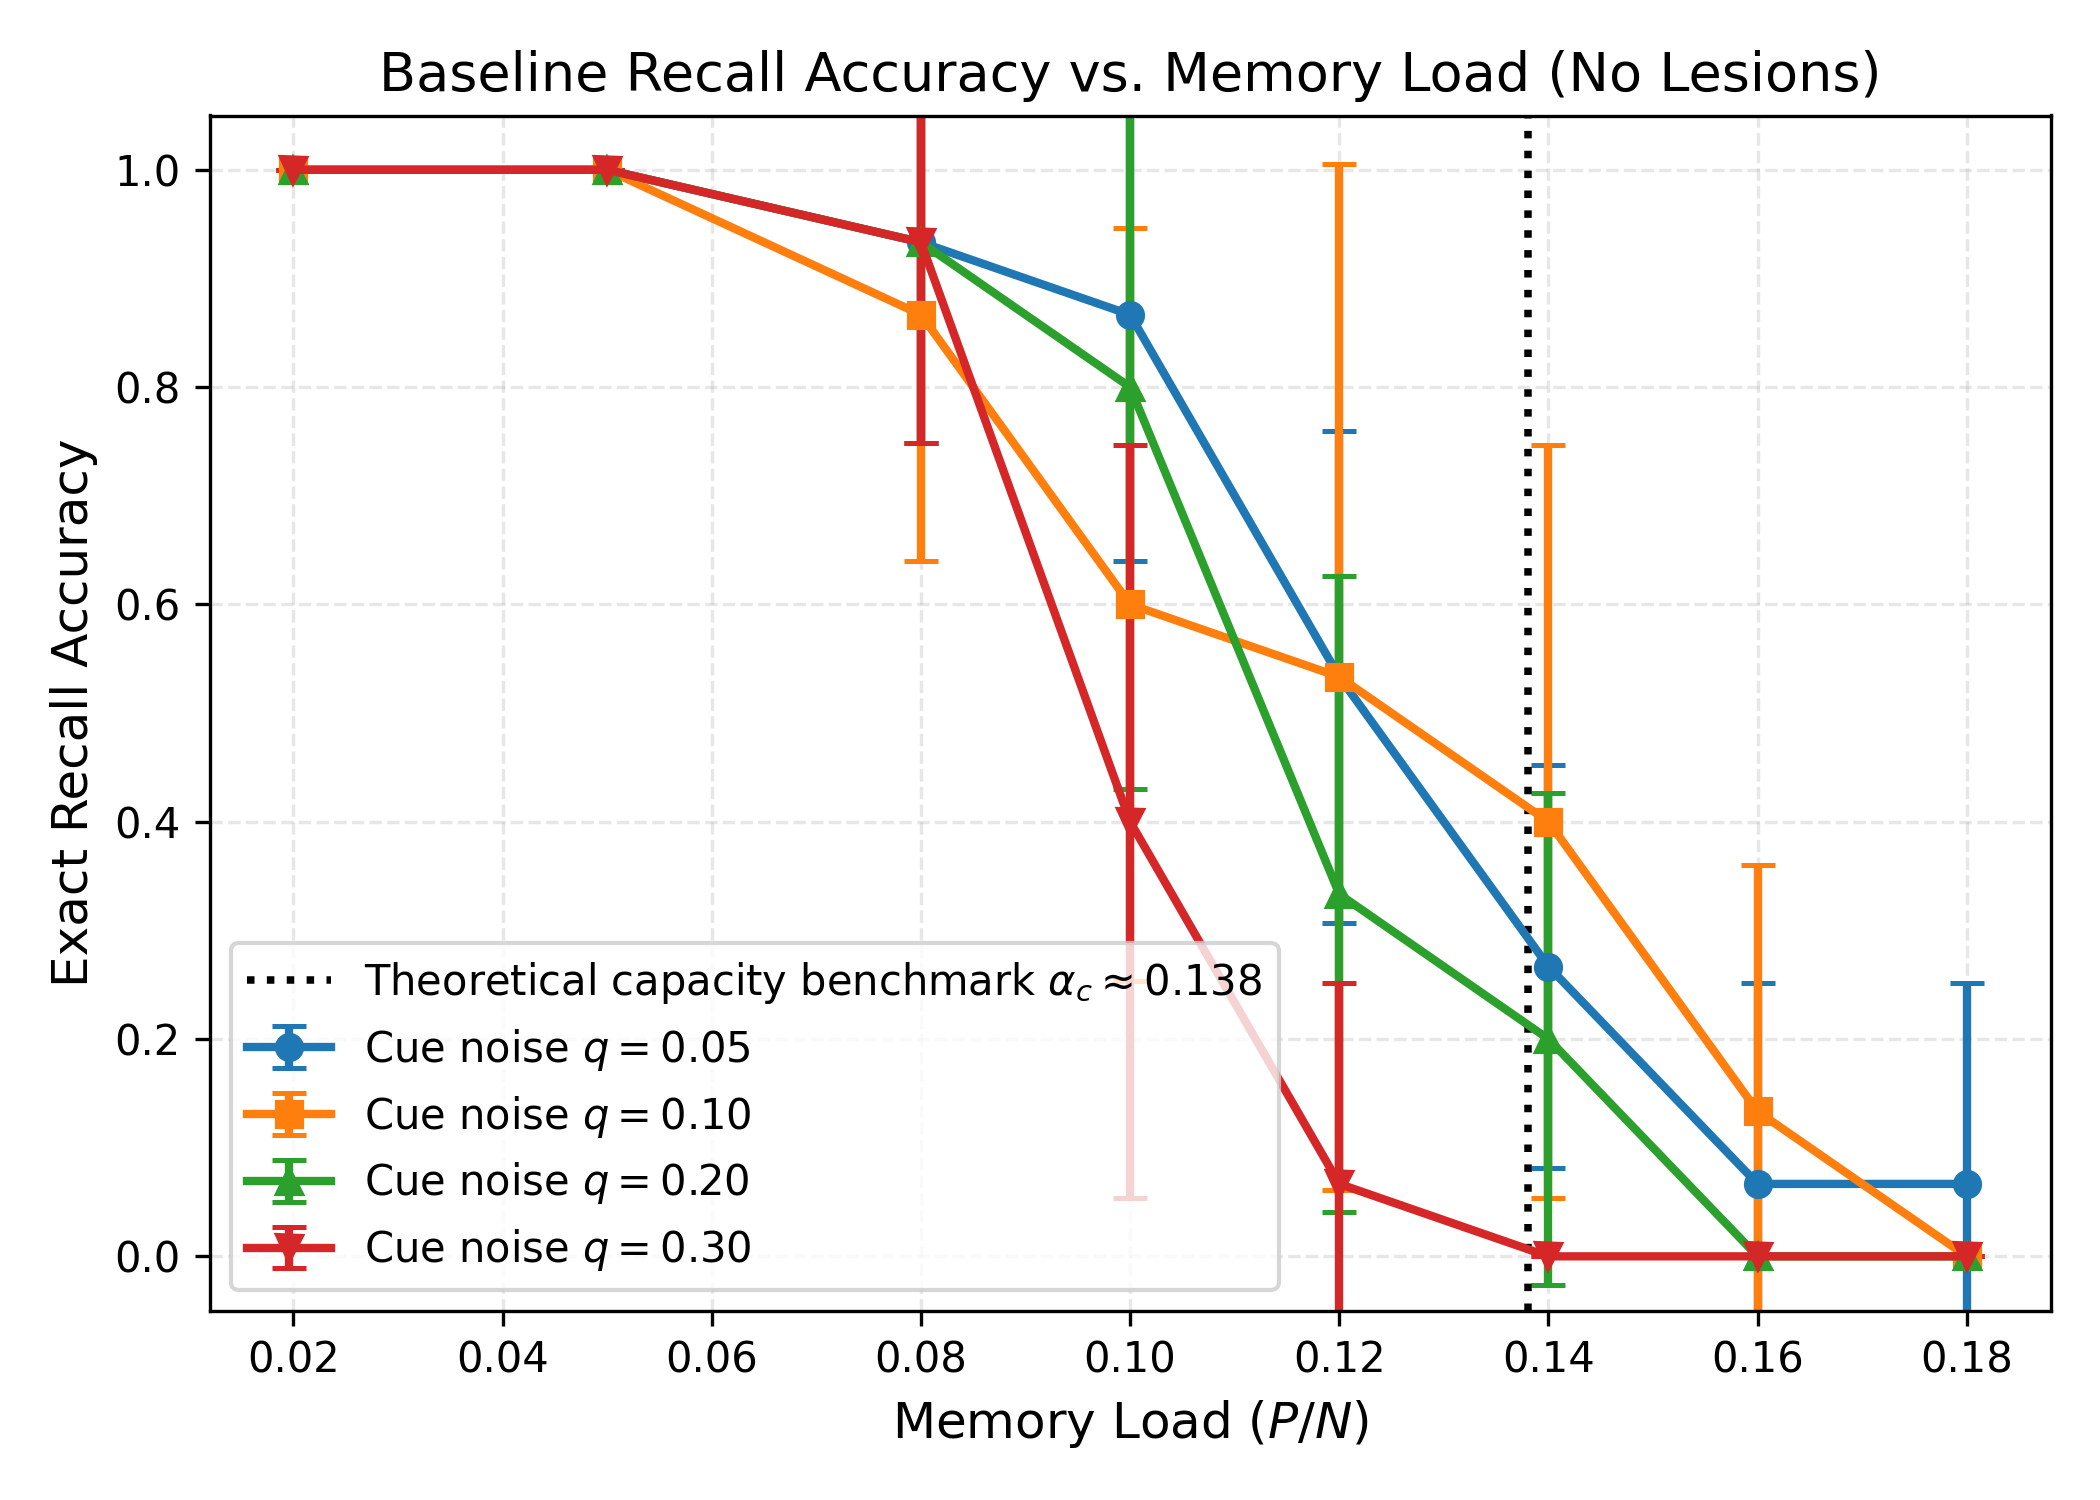
\includegraphics[width=0.66\textwidth]{figures/fig1_baseline_load_vs_accuracy.png}
    \caption{\textbf{Baseline Recall Accuracy vs. Memory Load ($f=0$).} Exact retrieval accuracy plotted against memory load $P/N$ across cue noise levels ($q \in [0.05, 0.30]$) with 95\% confidence intervals. The dotted line marks $\alpha_c \approx 0.138$.}
    \label{fig:baseline}
\end{figure}

\subsubsection{Synaptic Lesions and Cognitive Reserve (RQ2)}
Figure~\ref{fig:lesions} and Table~\ref{tab:load_lesion} demonstrate a profound interaction between memory load and lesion resilience. Under low memory load ($P/N = 0.05$, $P=20$):
\begin{itemize}
    \item Exact recall remains at \textbf{100\%} across lesion fractions $f = 0.00, 0.05, 0.10, 0.20,$ and \textbf{0.30}.
    \item Even when \textbf{50\% of all synapses are randomly deleted}, the network achieves an exact recall accuracy of \textbf{66.7\%} (with Hamming similarity exceeding 95\%).
\end{itemize}
Conversely, when the network operates near capacity ($P/N = 0.14$, $P=56$):
\begin{itemize}
    \item Undamaged baseline accuracy is already compromised at 40.0\%.
    \item A mild 10\% lesion cuts accuracy to 13.3\%.
    \item At 20\% lesions, recall collapses to \textbf{0.0\%}.
\end{itemize}
This divergence confirms Hypothesis 2: networks with spare capacity possess broad, deep attractor basins capable of absorbing substantial synaptic pruning before functional impairment occurs. The global two-dimensional phase space is summarized in Figure~\ref{fig:heatmap}.

\begin{figure}[H]
    \centering
    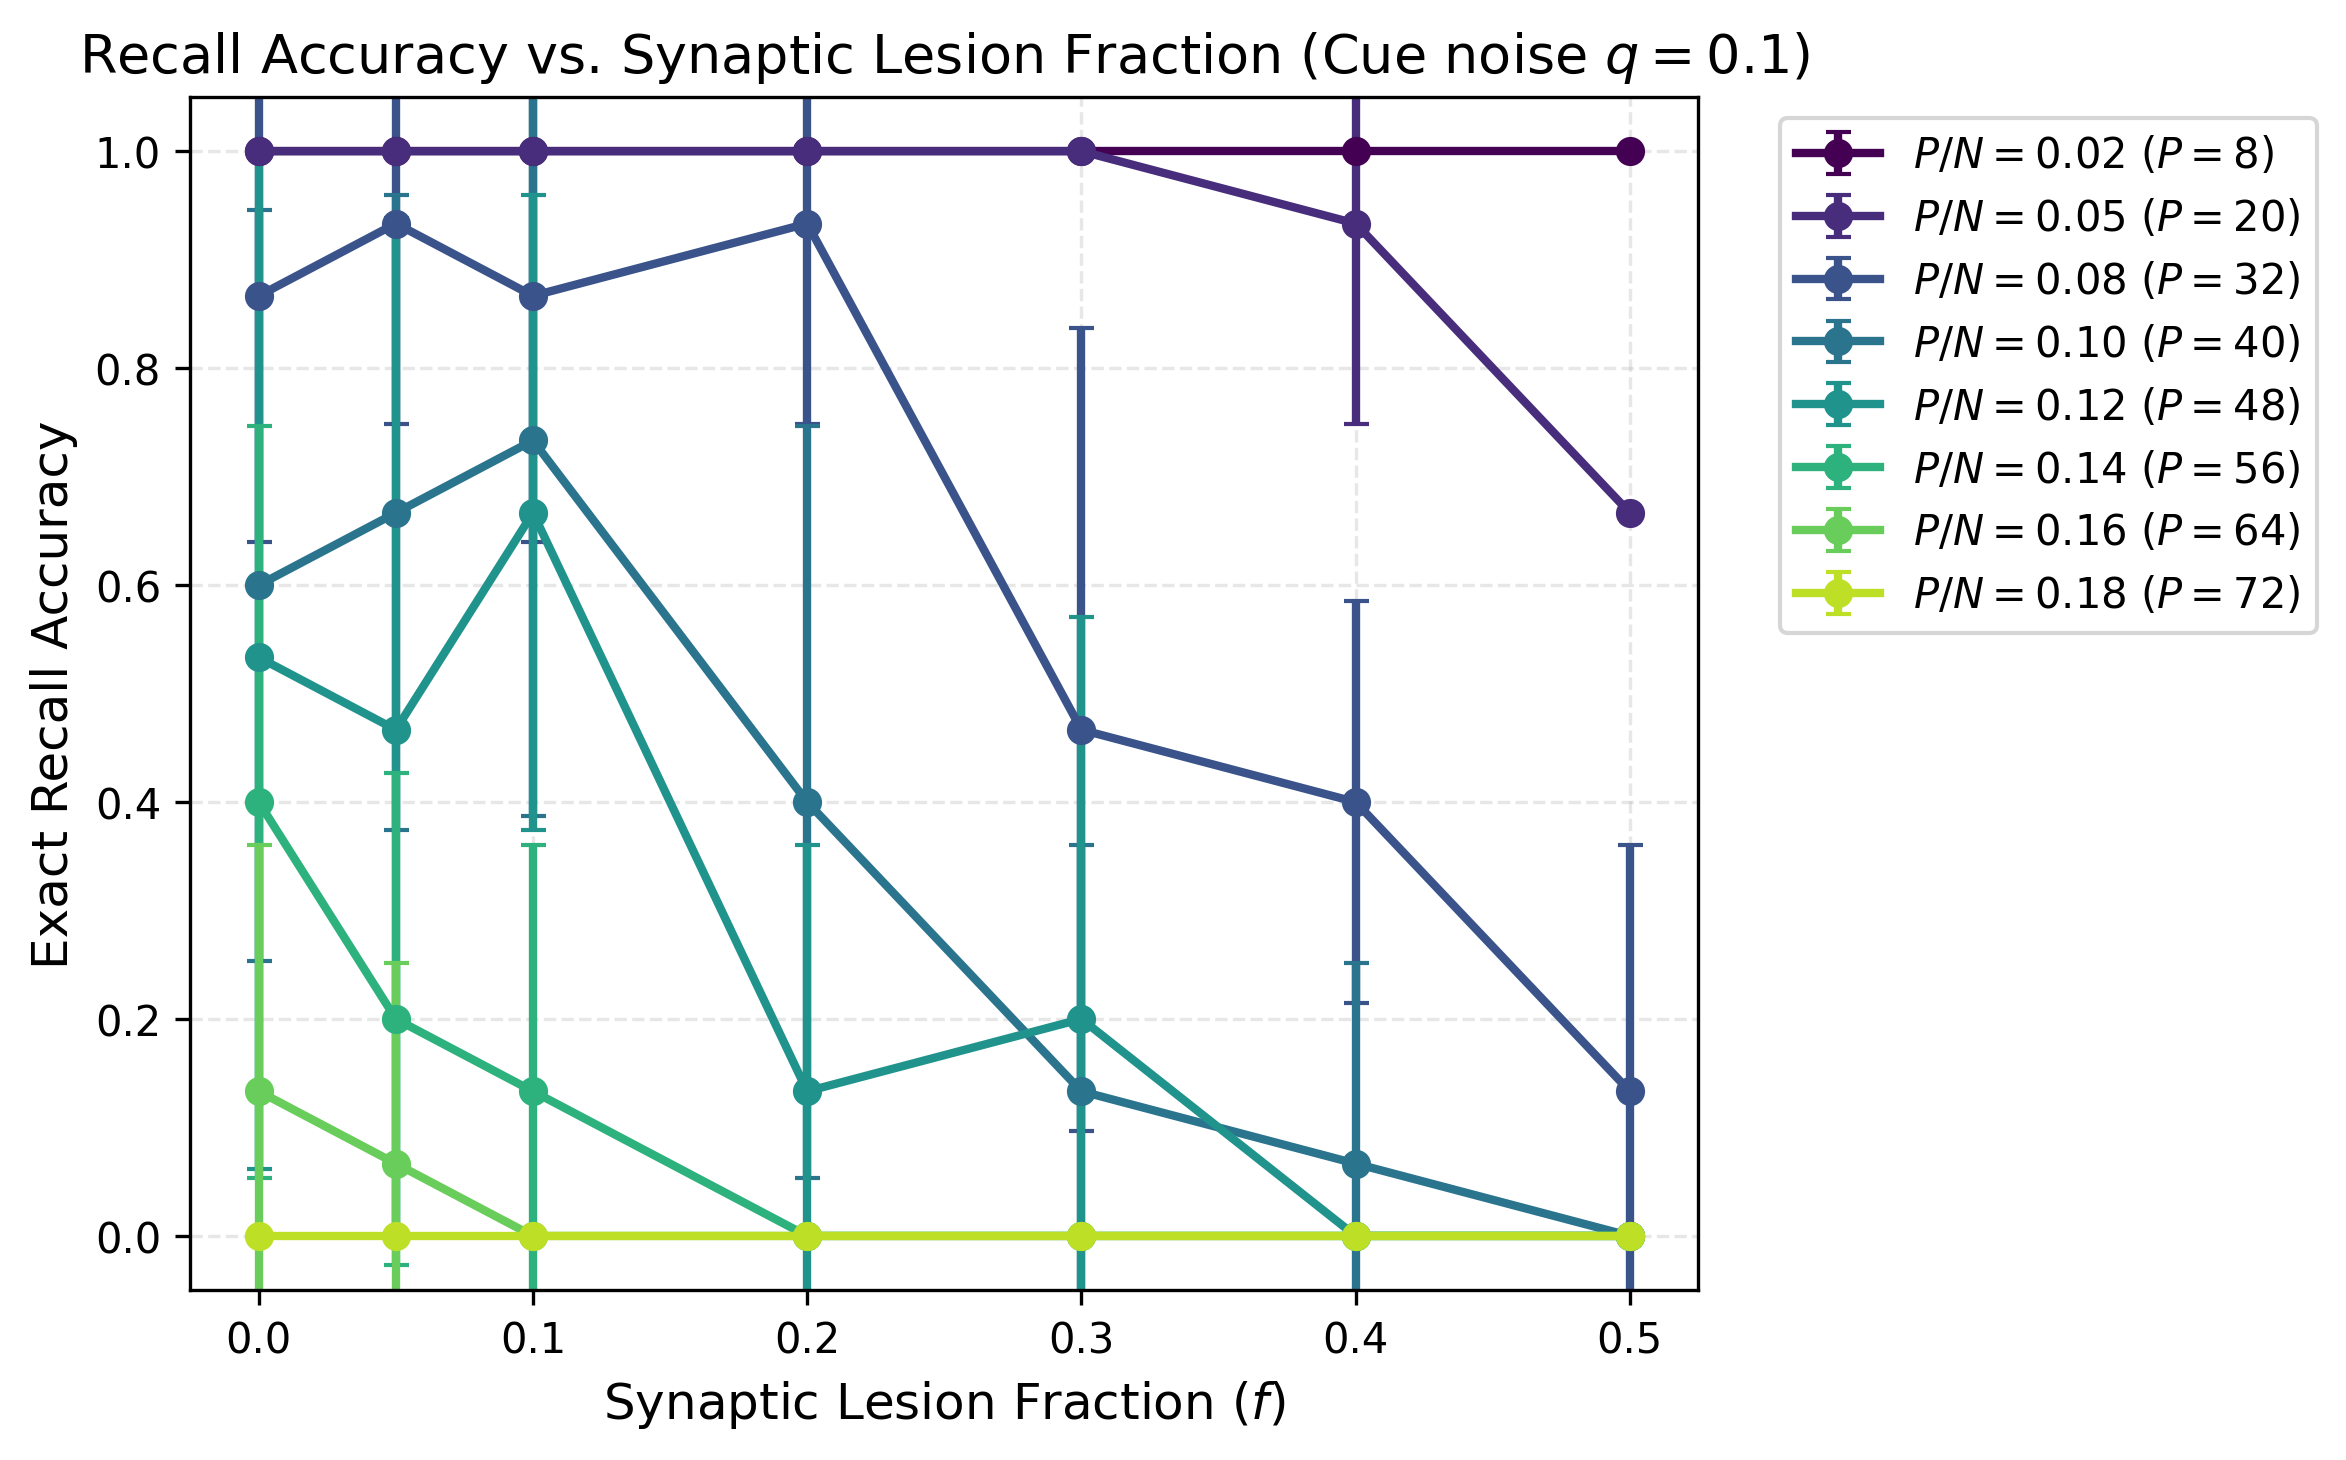
\includegraphics[width=0.72\textwidth]{figures/fig2_lesions_vs_accuracy.png}
    \caption{\textbf{Recall Accuracy vs. Synaptic Lesion Fraction.} Performance degradation curves across memory loads ($P/N \in [0.02, 0.18]$) under cue noise $q=0.10$. Low-load networks show a resilience plateau up to $f=0.30$.}
    \label{fig:lesions}
\end{figure}

\begin{table}[H]
\centering
\small
\caption{\textbf{Interaction of Memory Load and Synaptic Lesions ($q=0.10$).} Mean exact recall [$\pm 95\%$ CI].}
\label{tab:load_lesion}
\begin{tabular}{lccccc}
\toprule
\textbf{Memory Load ($P/N$)} & \textbf{$f = 0.00$} & \textbf{$f = 0.10$} & \textbf{$f = 0.20$} & \textbf{$f = 0.30$} & \textbf{$f = 0.50$} \\
\midrule
$P/N = 0.02$ ($P=8$)   & $1.000 \pm 0.00$ & $1.000 \pm 0.00$ & $1.000 \pm 0.00$ & $1.000 \pm 0.00$ & $0.933 \pm 0.13$ \\
$P/N = 0.05$ ($P=20$)  & $1.000 \pm 0.00$ & $1.000 \pm 0.00$ & $1.000 \pm 0.00$ & $1.000 \pm 0.00$ & $0.667 \pm 0.37$ \\
$P/N = 0.08$ ($P=32$)  & $0.867 \pm 0.23$ & $0.800 \pm 0.35$ & $0.733 \pm 0.35$ & $0.467 \pm 0.37$ & $0.067 \pm 0.13$ \\
$P/N = 0.10$ ($P=40$)  & $0.600 \pm 0.35$ & $0.467 \pm 0.37$ & $0.200 \pm 0.28$ & $0.067 \pm 0.13$ & $0.000 \pm 0.00$ \\
$P/N = 0.14$ ($P=56$)  & $0.400 \pm 0.35$ & $0.133 \pm 0.23$ & $0.000 \pm 0.00$ & $0.000 \pm 0.00$ & $0.000 \pm 0.00$ \\
$P/N = 0.18$ ($P=72$)  & $0.000 \pm 0.00$ & $0.000 \pm 0.00$ & $0.000 \pm 0.00$ & $0.000 \pm 0.00$ & $0.000 \pm 0.00$ \\
\bottomrule
\end{tabular}
\end{table}

\begin{figure}[H]
    \centering
    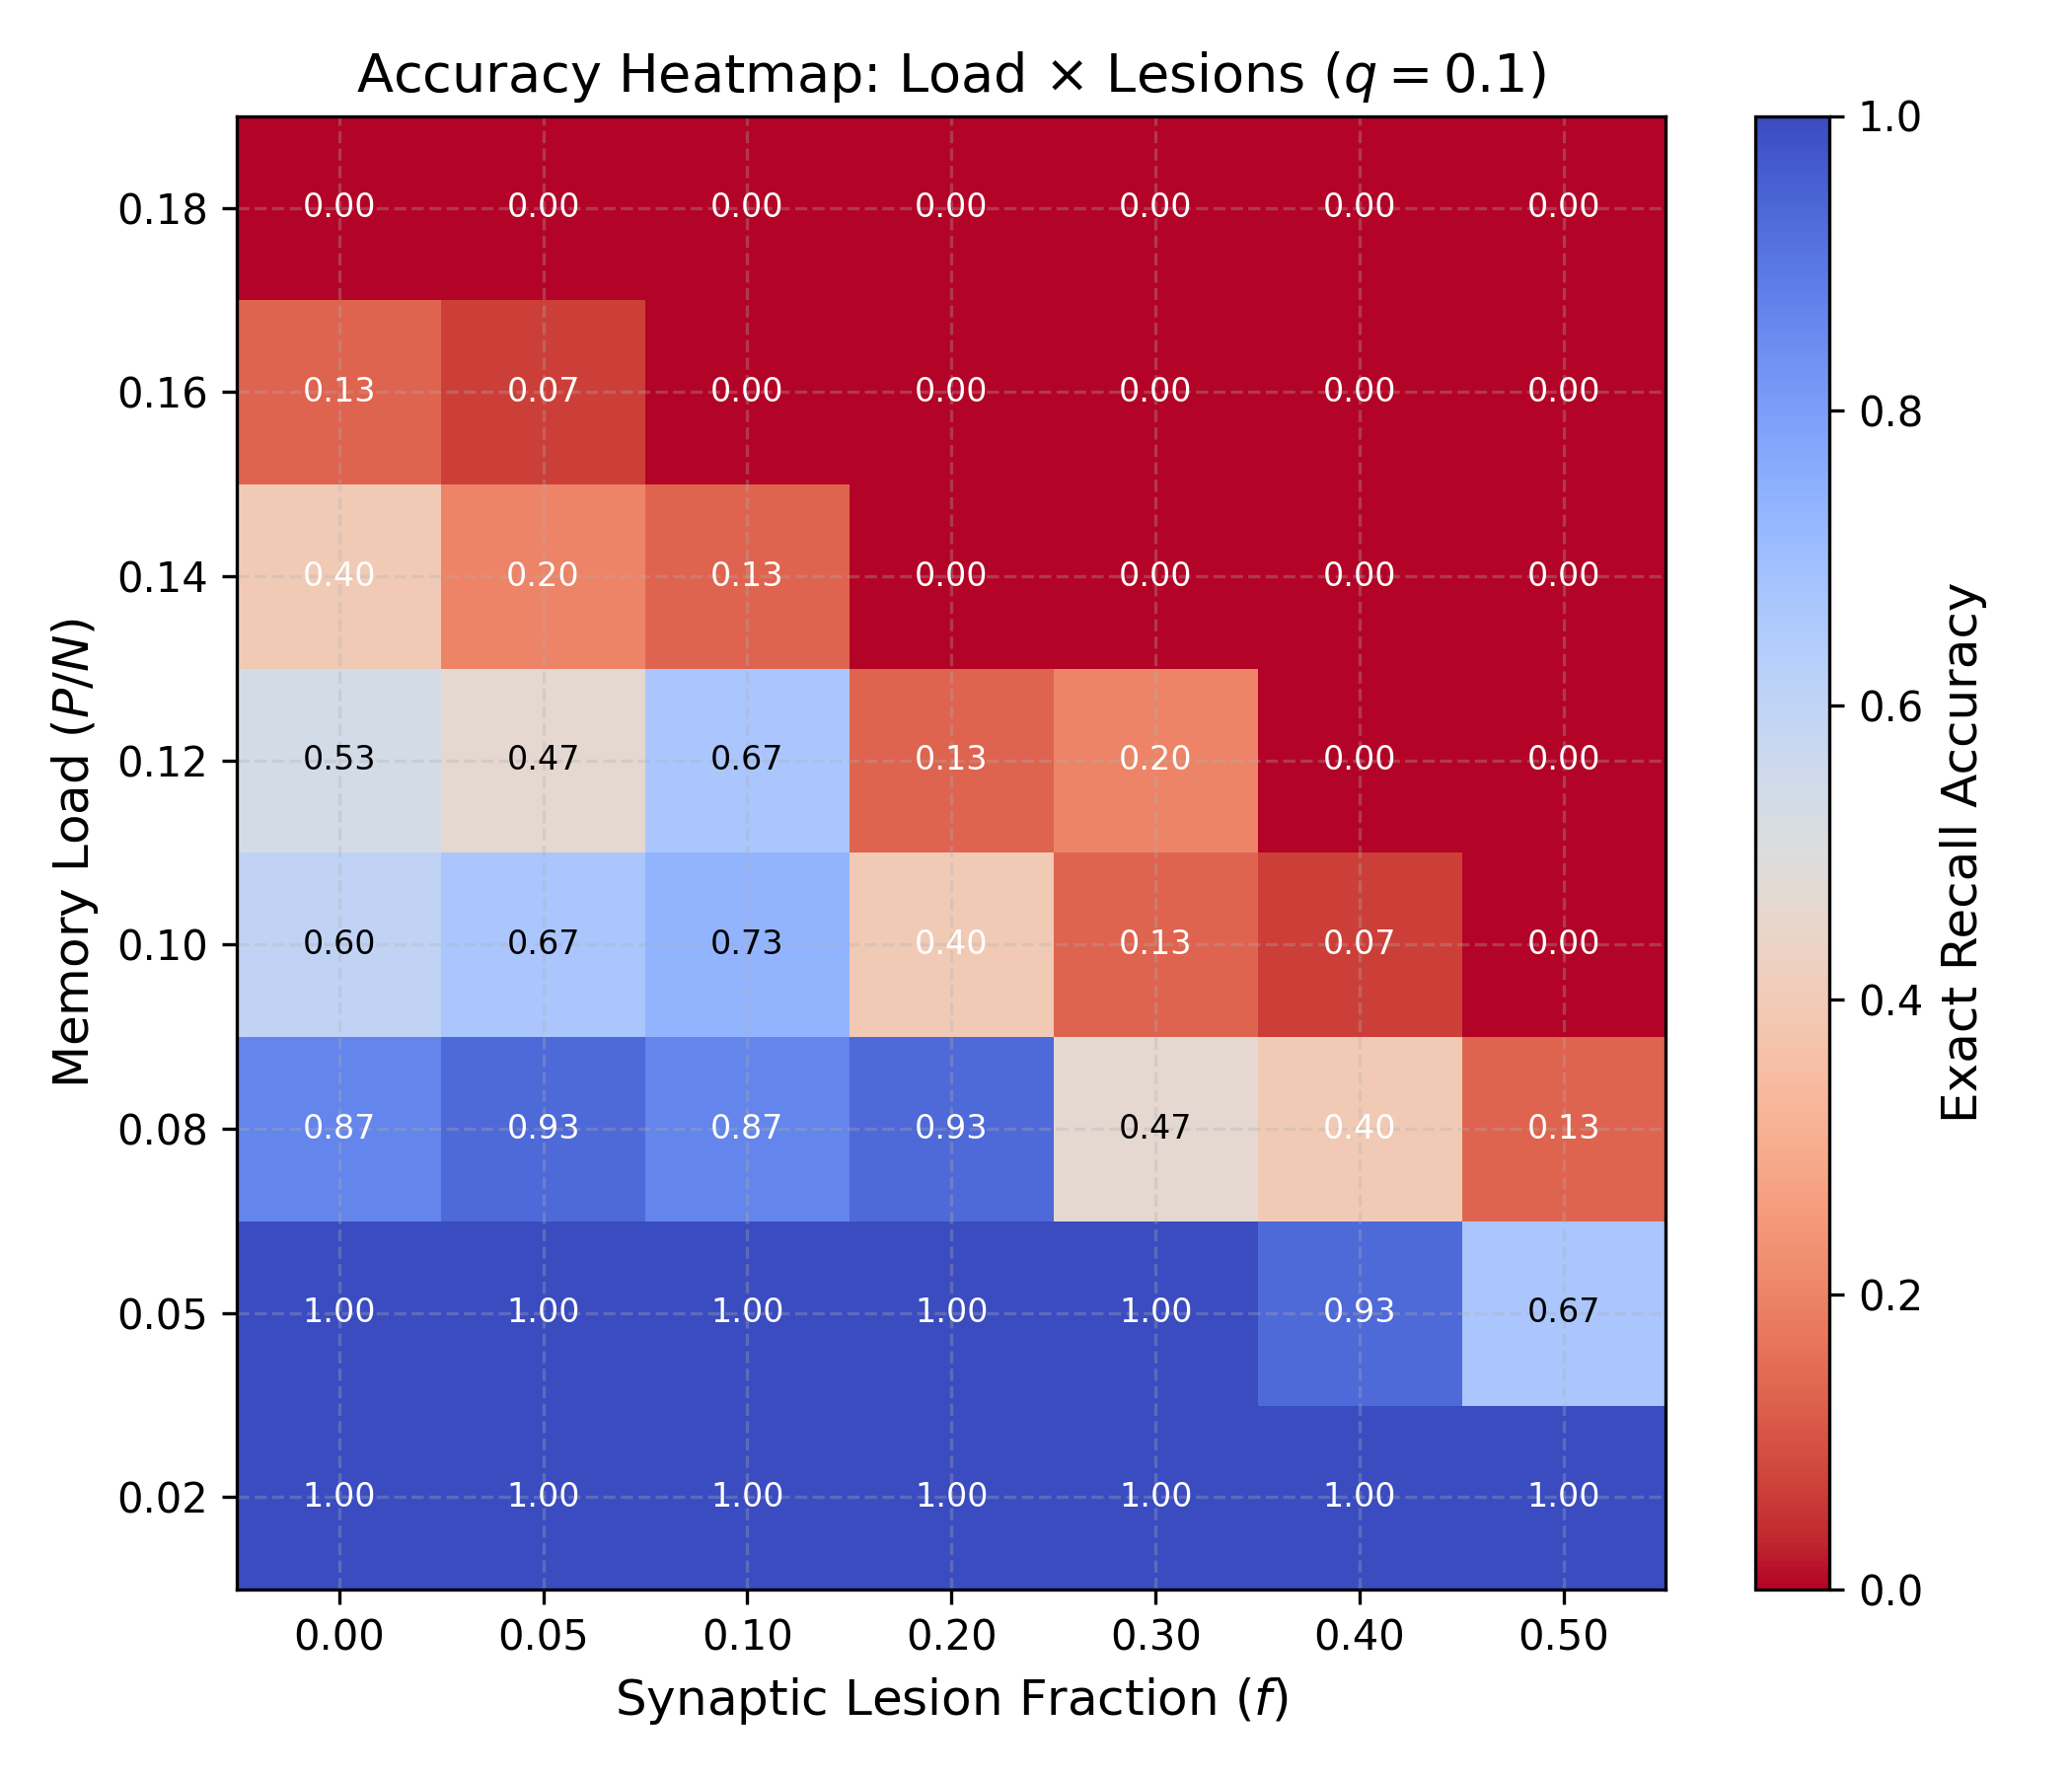
\includegraphics[width=0.62\textwidth]{figures/fig3_heatmap_load_vs_lesion.png}
    \caption{\textbf{Two-Dimensional Phase Space of Recall Accuracy.} Heatmap of exact recall accuracy over memory load ($P/N \in [0.02, 0.18]$) versus lesion fraction ($f \in [0.00, 0.50]$) at cue noise $q=0.10$.}
    \label{fig:heatmap}
\end{figure}

\subsubsection{Composition of Retrieval Errors (RQ3)}
Figure~\ref{fig:composition} breaks down retrieval outcomes across memory loads for intact ($f=0.00$), moderately lesioned ($f=0.20$), and heavily lesioned ($f=0.40$) networks. Errors are \textbf{not} caused by confusion with other stored memories ($< 2.5\%$ across all conditions). Non-convergence remained low ($< 15\%$), occurring only under extreme lesions. Instead, the overwhelming majority of failed recall trials settled into \textbf{Stable Spurious States}:
\begin{itemize}
    \item In an intact network at high load ($P/N=0.14$), 60.0\% of trials terminated in stable spurious attractors.
    \item Under moderate damage ($f=0.20$), stable spurious attractors captured \textbf{93.3\%} of all trials.
\end{itemize}
This supports Hypothesis 3: damage and overload warp the energy landscape, sculpting stable false attractors that trap retrieval trajectories.

\begin{figure}[H]
    \centering
    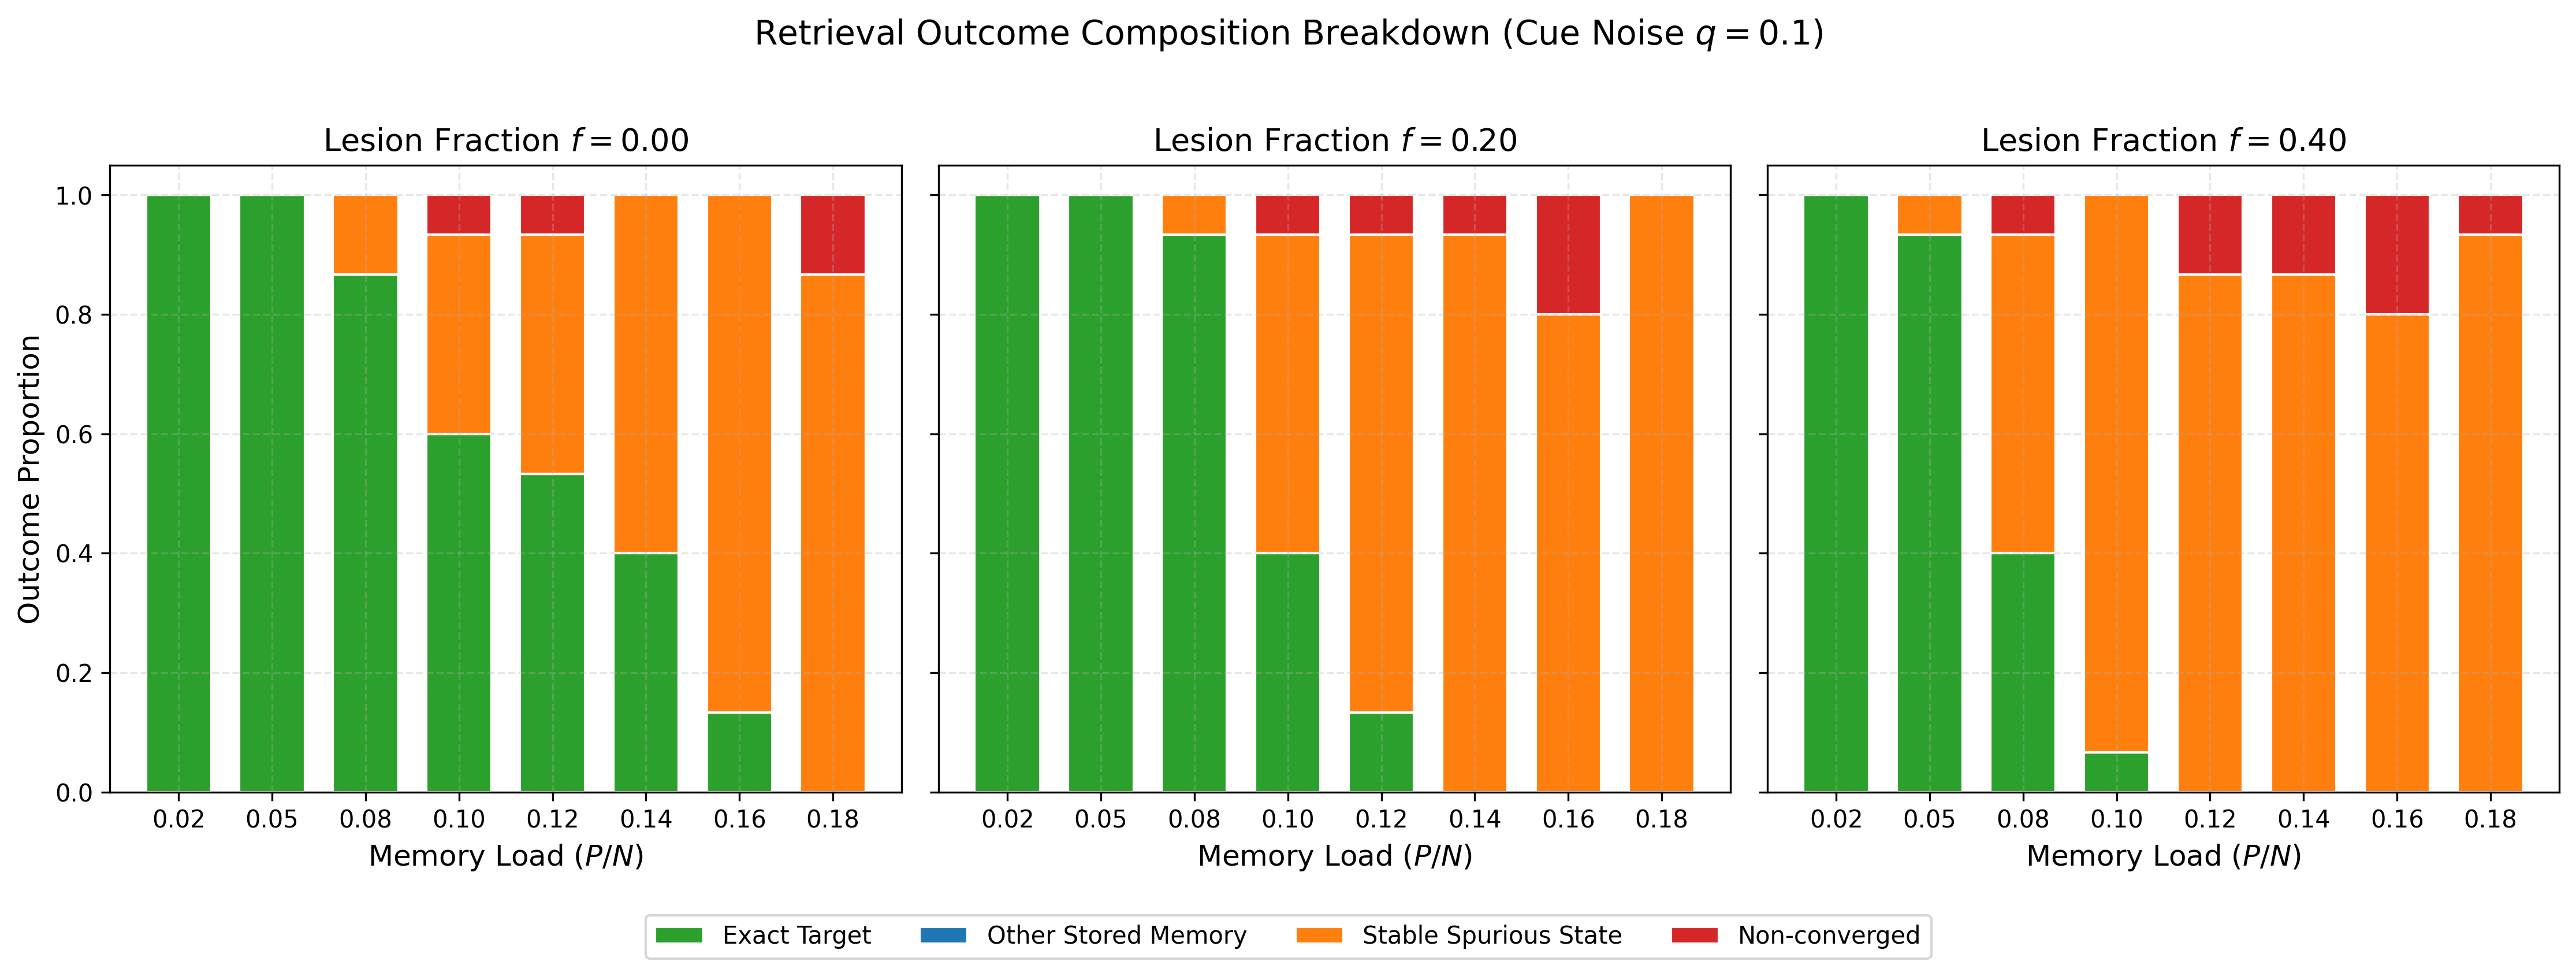
\includegraphics[width=0.88\textwidth]{figures/fig4_outcome_composition.png}
    \caption{\textbf{Retrieval Outcome Composition.} Stacked proportion of exact target recall (green), other stored memories (blue), stable spurious states (orange), and non-converged runs (red) across memory loads for $f=0.00, 0.20, 0.40$ ($q=0.10$).}
    \label{fig:composition}
\end{figure}

\subsubsection{Cue Corruption and Basin Boundary Dynamics (RQ4)}
Figure~\ref{fig:cue_noise} depicts the interaction between cue noise $q$ and synaptic damage. When the cue is lightly corrupted ($q=0.05$), the network reconstitutes the memory even under 30\% lesions. However, as cue noise increases to $q=0.30$, performance drops sharply. Severe cue noise initiates the state vector closer to basin boundaries, leaving retrieval vulnerable to lesion-induced basin contraction.

\begin{figure}[H]
    \centering
    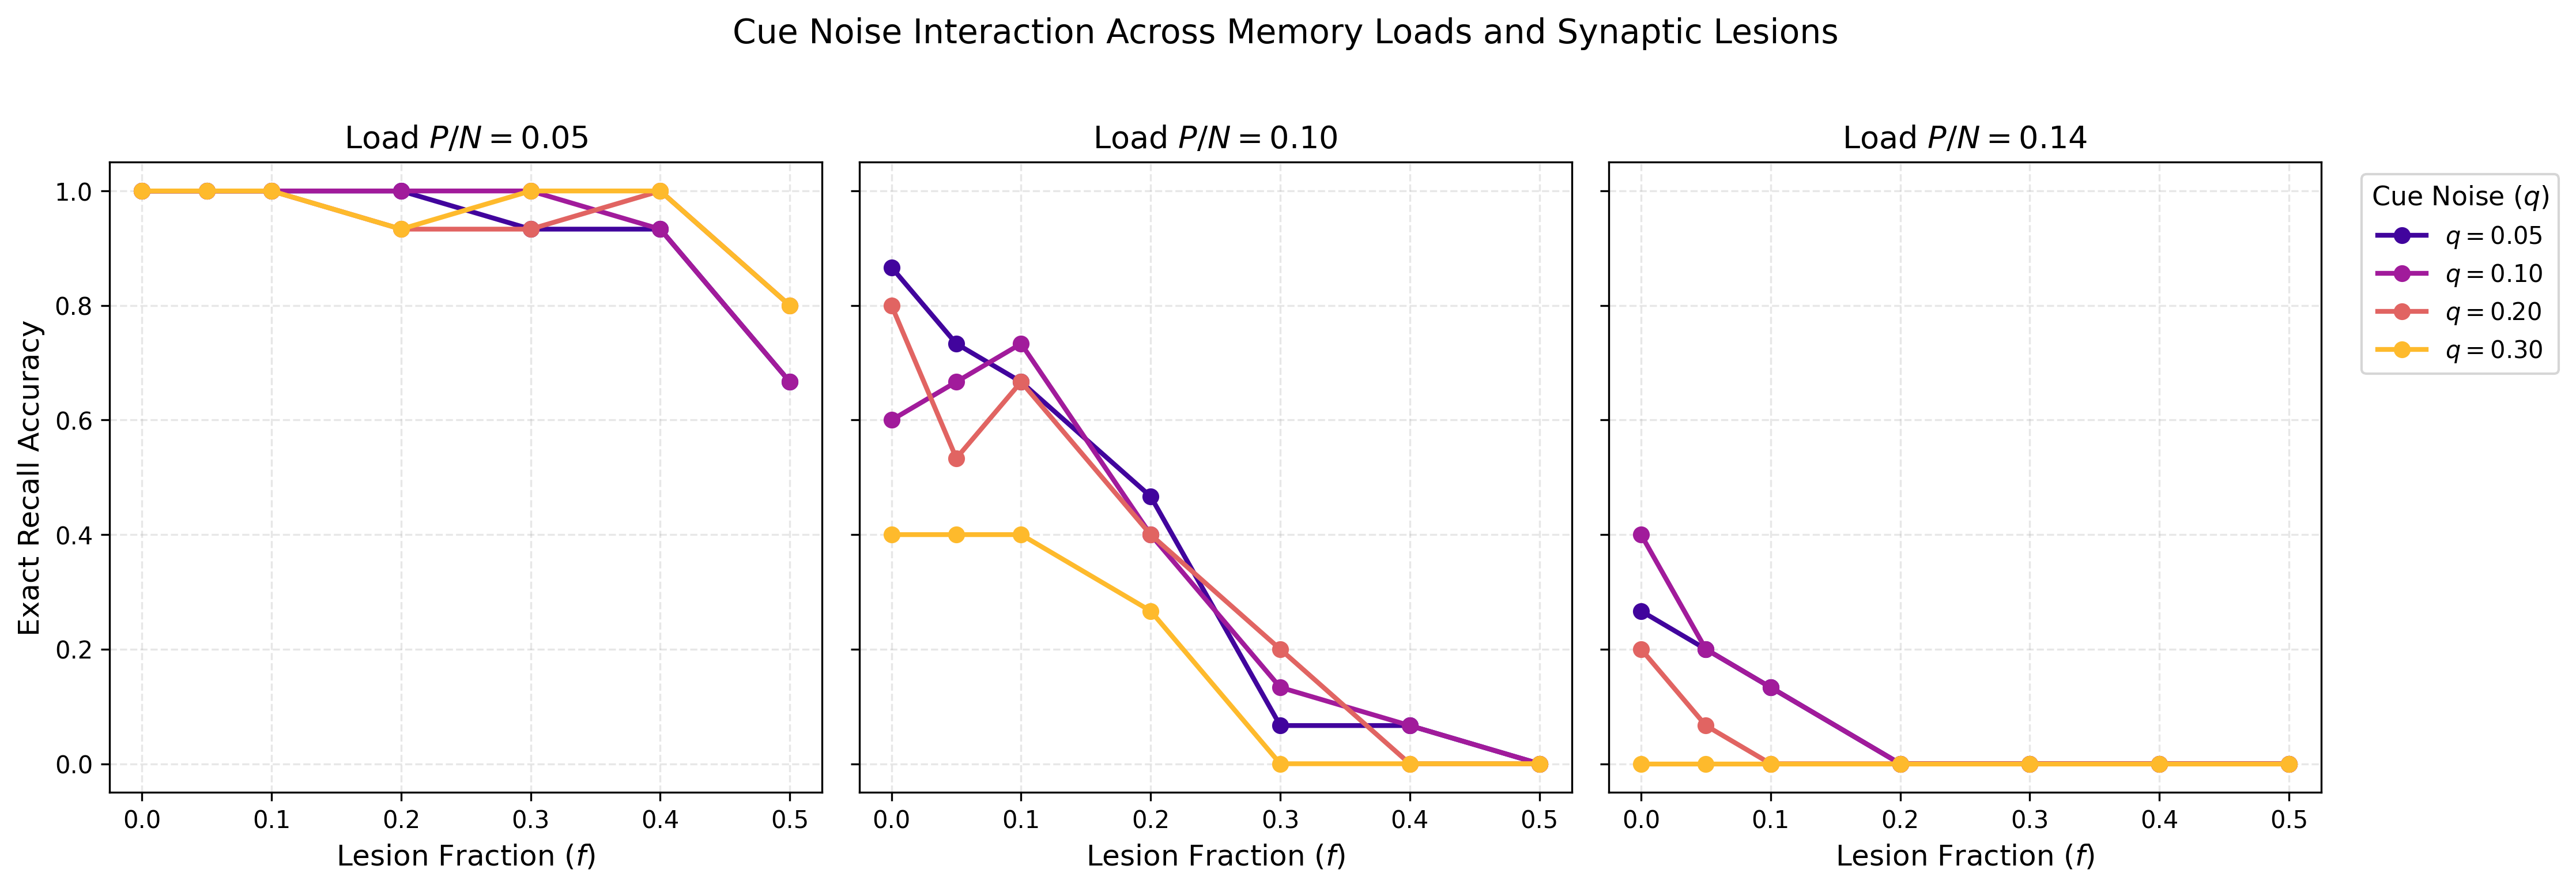
\includegraphics[width=0.88\textwidth]{figures/fig5_cue_corruption_interaction.png}
    \caption{\textbf{Cue Corruption Interaction Across Memory Loads.} Recall accuracy versus synaptic lesion fraction for cue noise probabilities ($q \in [0.05, 0.30]$) across low ($P/N=0.05$), medium ($P/N=0.10$), and high ($P/N=0.14$) loads.}
    \label{fig:cue_noise}
\end{figure}

\subsection{Extension and Comparison: Naturalistic MNIST vs. Synthetic Patterns}
\noindent\textbf{The Question It Answers:} \textit{How do natural spatial correlations and non-orthogonal feature overlap alter associative capacity and the nature of false recall?}

To test ecological validity, we extended the architecture to store binarized handwritten digits from MNIST ($N=784$, $28 \times 28$ pixels) and compared them with synthetic orthogonal patterns ($N=784$). As shown in Table~\ref{tab:mnist} and Figure~\ref{fig:mnist}:
\begin{itemize}
    \item \textbf{Exact Recall:} While synthetic patterns maintain 100\% recall across $P=2$ through $P=20$, MNIST collapses from 100\% at $P=2$ to \textbf{0\% exact recall at $P \ge 4$}.
    \item \textbf{Hamming Similarity:} Despite zero exact recall, MNIST maintains high normalized Hamming similarity ($\sim 88\% - 94\%$).
\end{itemize}
Handwritten digits share dense spatial correlations ($\mathbb{E}[\xi_i^\mu \xi_j^\mu] > 0$) and a heavy background bias. Under standard Hebbian learning, mutual correlation creates massive cross-talk that destroys isolated individual attractors. Instead, the network settles into a \textbf{prototypical mixture state}---reconstructing the coarse digit outline while blending overlapping strokes.

\begin{table}[H]
\centering
\small
\caption{\textbf{MNIST vs. Synthetic Patterns ($N=784$, Undamaged $f=0$, $q=0.10$).}}
\label{tab:mnist}
\begin{tabular}{lcccc}
\toprule
\textbf{Stored Patterns ($P$)} & \textbf{Synthetic Acc.} & \textbf{MNIST Acc.} & \textbf{Synthetic Sim.} & \textbf{MNIST Sim.} \\
\midrule
$P = 2$  & $1.000$ & $1.000$ & $1.000$ & $1.000$ \\
$P = 4$  & $1.000$ & $0.000$ & $1.000$ & $0.939$ \\
$P = 6$  & $1.000$ & $0.000$ & $1.000$ & $0.896$ \\
$P = 8$  & $1.000$ & $0.000$ & $1.000$ & $0.890$ \\
$P = 10$ & $1.000$ & $0.000$ & $1.000$ & $0.876$ \\
$P = 20$ & $1.000$ & $0.000$ & $1.000$ & $0.878$ \\
\bottomrule
\end{tabular}
\end{table}

\begin{figure}[H]
    \centering
    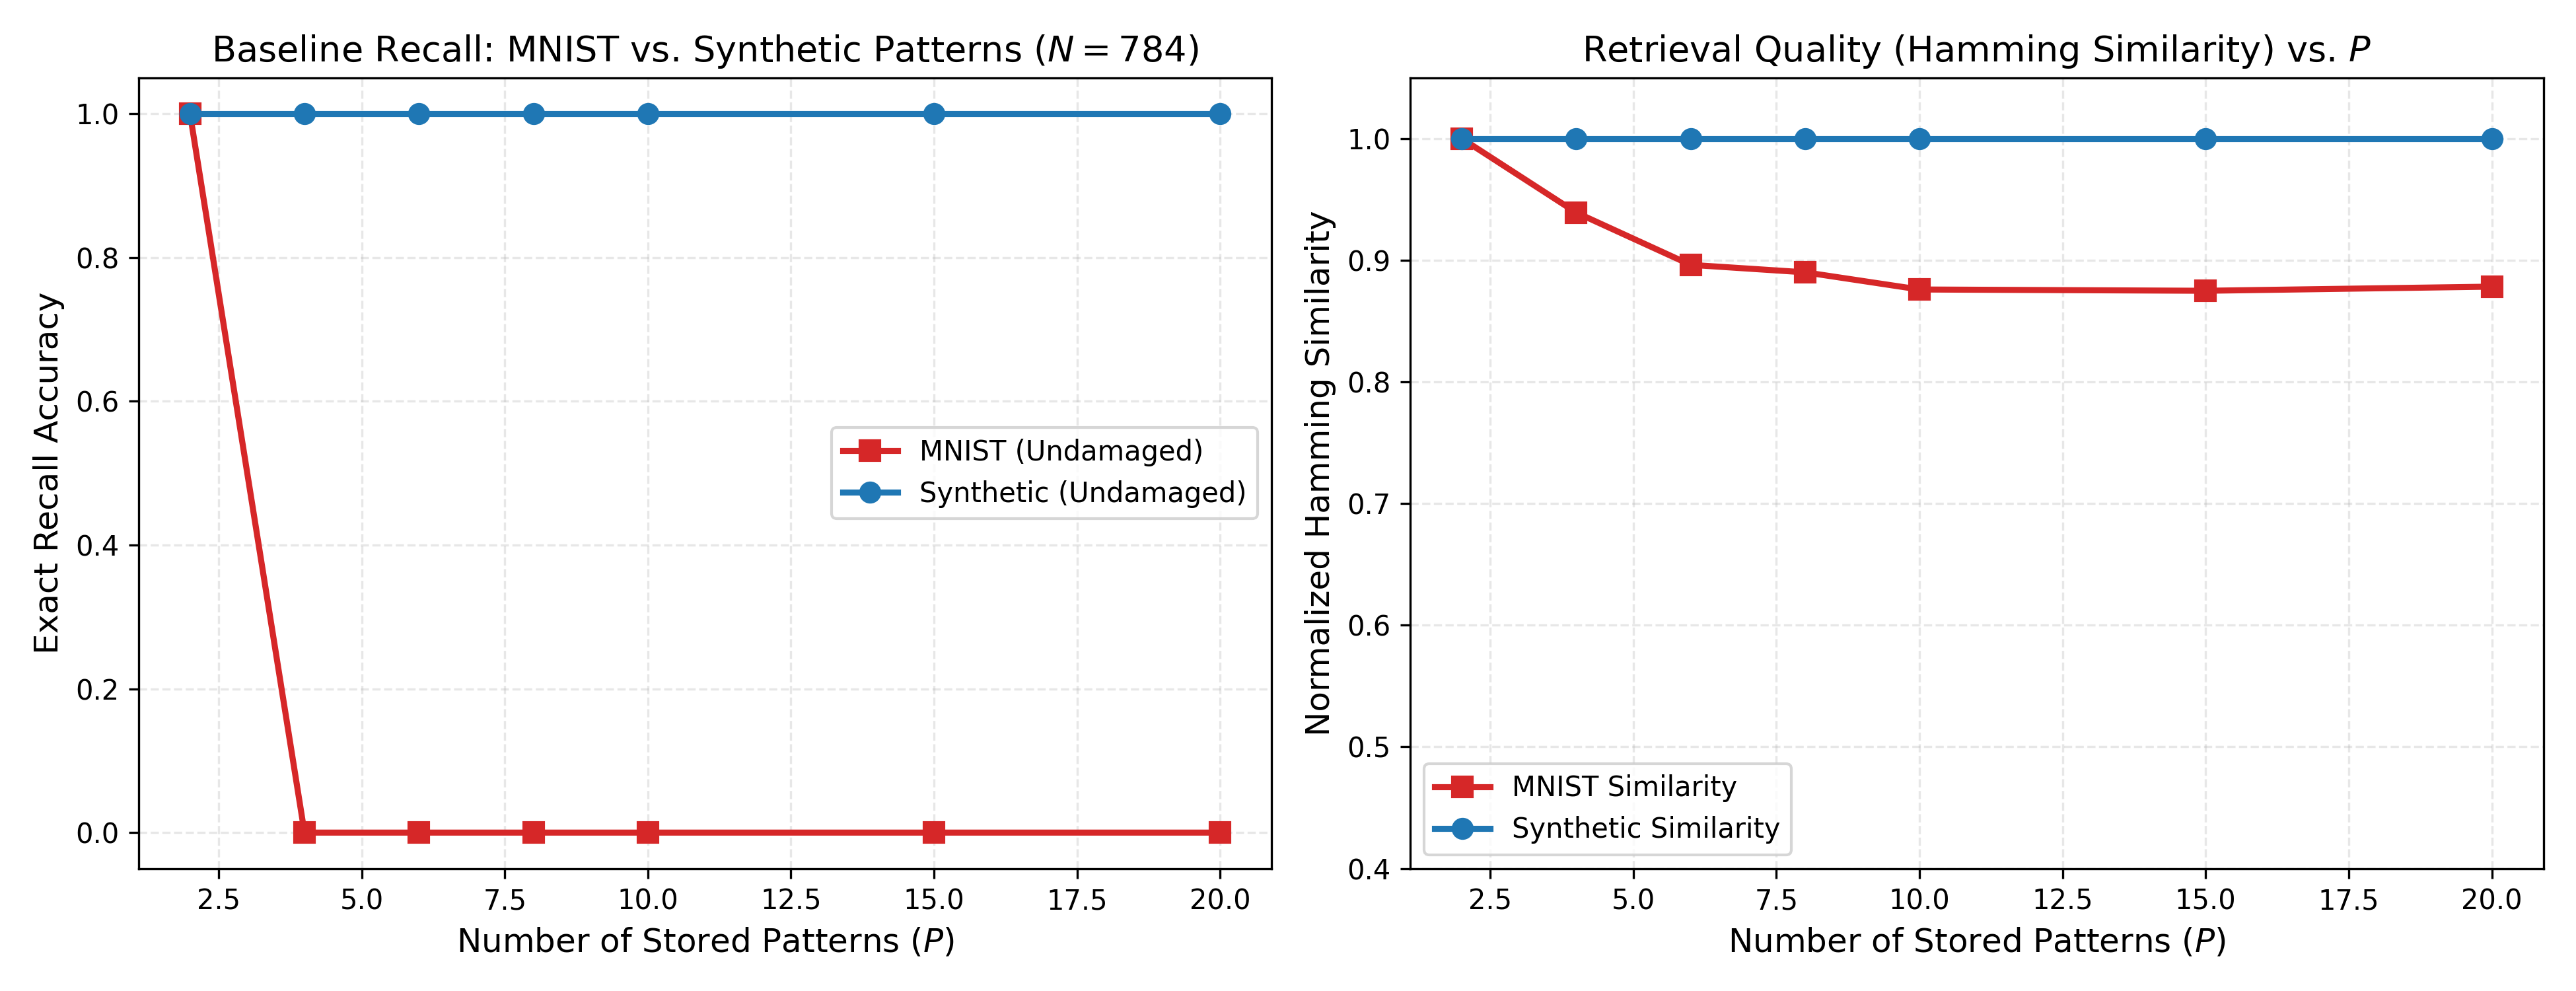
\includegraphics[width=0.82\textwidth]{figures/fig7_mnist_vs_synthetic.png}
    \caption{\textbf{MNIST vs. Synthetic Pattern Performance ($N=784$).} Left panel: Exact recall accuracy versus $P$. Right panel: Normalized Hamming similarity showing that while exact recall collapses for MNIST, pattern completion maintains $\sim 90\%$ semantic feature overlap.}
    \label{fig:mnist}
\end{figure}

\section{Discussion}

\subsection{Interpretation of Findings}

\subsubsection{What the Model Explains: Cognitive Reserve and Spurious Attractors}
Unlike digital memory architectures, where a single severed connection induces fatal crashes, distributed attractor networks degrade gracefully. Crucially, our results provide a mechanistic grounding for the \textit{cognitive reserve hypothesis} \cite{stern2002, stern2012}. Clinicians observe that patients with high cognitive reserve endure substantial Alzheimer's neuropathology before expressing clinical dementia. In our model, this corresponds directly to the resilience plateau in Figure~\ref{fig:lesions}: below capacity ($P/N = 0.05$), attractor basins are deep and broad, tolerating 30\% synaptic loss with zero behavioral deficit. Structural reserve emerges as a direct property of low inter-memory interference.

Furthermore, our error analysis reveals that memory failure is almost never random noise or confusion with another intact memory. Instead, over 93\% of retrieval failures converge to \textbf{stable spurious states}. In statistical physics, these represent odd-symmetry mixture attractors and spin-glass local minima \cite{amit1985}. In cognitive terms, the network does not ``erase'' memories; rather, synaptic damage warps the energy landscape, creating synthetic energy valleys. This offers a computational analogue for clinical confabulation and the Deese--Roediger--McDermott (DRM) false memory effect \cite{roediger1995}.

\subsubsection{Where the Model Fails}
The model fails when confronted with correlated, naturalistic stimuli (MNIST). Because basic Hebbian plasticity cannot decouple overlapping features, exact capacity collapses at $P=4$. Biological memory resolves this through hippocampal circuitry: the dentate gyrus performs sparse coding (pattern separation) before associations are stored in CA3.

\subsubsection{Alternative Explanation of the Findings}
Could the observed resilience and breakdown be explained without recurrent attractor dynamics? An alternative explanation is a \textbf{feedforward matched-filter / signal-to-noise ratio (SNR) model}. In a linear feedforward autoencoder, connection dropout degrades signal linearly proportional to $(1-f)$. Under an SNR model, one would expect a smooth, linear decrease in accuracy. However, our empirical data reveals a sharp non-linear step-function: accuracy remains flat at 100\% up to $f=0.30$, followed by a steep drop. This non-linear resilience is the definitive signature of recurrent attractor dynamics restoring corrupted states within an attraction basin.

\subsection{Limitations and Future Directions}
\textbf{Limitations:} The classical Hopfield model simplifies biological reality: biological synapses violate weight symmetry ($W_{ij} \ne W_{ji}$), obey Dale's Law (segregated excitation/inhibition), and feature sparse connectivity. Uniform random edge deletion also simplifies focal neuropathologies like tau tangles.

\textbf{Future Directions:} Future work should explore: (i) sparse pseudo-inverse learning to store correlated naturalistic patterns; (ii) asymmetric Dale-compliant architectures; and (iii) targeted topological lesions (e.g., pruning high-centrality hub neurons) to model specific neurodegenerative disease profiles.

\section{Contribution Statement}
\noindent\textbf{Author Contributions:} H.S. conceived the computational framework, formulated the mathematical models, developed the Python simulation codebase and unit test suite, executed parameter sweeps and MNIST extensions, performed statistical analyses, generated publication-quality figures, and authored the research manuscript.

\section{AI Use Disclosure}
\noindent\textbf{Disclosure:} Generative AI tooling (Google DeepMind Antigravity) was utilized as an assistive pair-programming environment to assist in structuring boilerplate Python multiprocessing routines, configuring LaTeX layout packages, and automating regression test execution. All conceptual hypotheses, experimental designs, algorithmic implementations, data interpretations, and final text writing were supervised and reviewed by the author.

\begin{thebibliography}{99}

\bibitem{hopfield1982}
J.~J. Hopfield, ``Neural networks and physical systems with emergent collective computational abilities,'' \emph{Proceedings of the National Academy of Sciences}, vol.~79, no.~8, pp. 2554--2558, 1982.

\bibitem{amit1985}
D.~J. Amit, H.~Gutfreund, and H.~Sompolinsky, ``Storing infinite numbers of patterns in a spin-glass model of neural networks,'' \emph{Physical Review Letters}, vol.~55, no.~14, pp. 1530--1533, 1985.

\bibitem{amit1987}
D.~J. Amit, H.~Gutfreund, and H.~Sompolinsky, ``Statistical mechanics of neural networks near saturation,'' \emph{Annals of Physics}, vol. 173, no.~1, pp. 30--67, 1987.

\bibitem{mceliece1987}
R.~J. McEliece, E.~C. Posner, E.~R. Rodemich, and S.~S. Venkatesh, ``The capacity of the Hopfield associative memory,'' \emph{IEEE Transactions on Information Theory}, vol.~33, no.~4, pp. 461--482, 1987.

\bibitem{abumostafa1985}
Y.~S. Abu-Mostafa and J.-M. St.~Jacques, ``Information capacity of the Hopfield model,'' \emph{IEEE Transactions on Information Theory}, vol.~31, no.~4, pp. 461--464, 1985.

\bibitem{stern2002}
Y.~Stern, ``What is cognitive reserve? Theory and research application of the reserve concept,'' \emph{Journal of the International Neuropsychological Society}, vol.~8, no.~3, pp. 448--460, 2002.

\bibitem{stern2012}
Y.~Stern, ``Cognitive reserve in ageing and Alzheimer's disease,'' \emph{The Lancet Neurology}, vol.~11, no.~11, pp. 1006--1012, 2012.

\bibitem{livingston2024}
G.~Livingston \emph{et~al.}, ``Dementia prevention, intervention, and care: 2024 report of the Lancet standing Commission,'' \emph{The Lancet}, vol. 404, no. 10452, pp. 572--628, 2024.

\bibitem{roediger1995}
H.~L. Roediger and K.~B. McDermott, ``Creating false memories: Remembering words not presented in lists,'' \emph{Journal of Experimental Psychology: Learning, Memory, and Cognition}, vol.~21, no.~4, pp. 803--814, 1995.

\bibitem{bartlett1932}
F.~C. Bartlett, \emph{Remembering: An Experimental and Social Study}. Cambridge: Cambridge University Press, 1932.

\bibitem{lecun1998}
Y.~LeCun, L.~Bottou, Y.~Bengio, and P.~Haffner, ``Gradient-based learning applied to document recognition,'' \emph{Proceedings of the IEEE}, vol.~86, no.~11, pp. 2278--2324, 1998.

\end{thebibliography}

\end{document}
